\section{Stima intervallare}

\subsection{Credibility intervall (bayesiano) e Confidence interval (frequentista)}

\begin{frame}[fragile]{Bayesian credibility Interval}
\begin{block}{Credibility (della posterior)}
\begin{align*}
&\cred{(x)}=\int_{\mu\in\inf(x)}\Pi(\mu|x)\,d\mu=\int_{\mu\inf(x)}\frac{\prob{(x|\mu)}\prob{(\mu)}}{\int\,d\mu}\,d\mu>\cl{}\\
&
\end{align*}
\end{block}
\begin{block}{Ordinamento}
\begin{picture}(100,130)
\put(20,20){
\begin{tikzpicture}[scale=0.4]
\def\basefunc{exp(-(x-1)^2)}
        \begin{axis}[title={central},name=central,samples=50,ymin=0,xmin=-2,xmax=4,xlabel={$m$},ylabel={$\prob{(m|x_0)}$}]
        \addplot gnuplot [no marks,domain={-2:0}]{\basefunc} \closedcycle; 
        \addplot gnuplot [no marks,domain={2:4}]{\basefunc} \closedcycle; 
        \addplot gnuplot [black,thick,fill=grey,smooth,no marks,domain={0:2}]{\basefunc} \closedcycle;
        \node (unomenocl) at (axis cs:-1,0.3) {$1-\frac{\alpha}{2}$};
        \end{axis}
        \begin{axis}[title={upper limit}, at={($(central)+(4.5cm,-3cm)$)},name=upper,samples=50,ymin=0,xmin=-2,xmax=4,xlabel={$m$},ylabel={$\prob{(m|x_0)}$}]
        \addplot gnuplot [no marks,fill=grey,domain={-2:2}]{\basefunc} \closedcycle; 
        \addplot gnuplot [black,thick,smooth,no marks,domain={2:4}]{\basefunc};   
        \end{axis}
        \edef\oprob{0.47}
        \begin{axis}[at={($(upper)+(4.5cm,-3cm)$)}, title={probability order},name=central,samples=50,ymin=0,xmin=-2,xmax=4,xlabel={$m$},ylabel={$\prob{(m|x_0)}$}]
        \addplot[name path=prob] gnuplot[grey,thick,smooth,no marks]{\oprob};
        \addplot[name path=gauss] gnuplot[black,thick,smooth,no marks]{\basefunc};
        \path [name intersections={of=gauss and prob ,by={Pa,Pb}}];
        \node[above left] at (Pa) {$x_-$} node[above right] at (Pb) {$x_+$};
        \pgfkeys{/pgf/fpu=true}
        \pgfmathparse{1-sqrt(-ln(\oprob))}
        \def\xleft{\pgfmathresult}
        \pgfmathparse{1+sqrt(-ln(\oprob))}
        \def\xright{\pgfmathresult}
        \pgfmathparse{1+sqrt(-ln(\oprob))}
        \pgfkeys{/pgf/fpu=false}
        \addplot gnuplot [no marks,fill=grey,domain={0.13:1.87}]{\basefunc} \closedcycle; 
        \node (unomenocl) at (axis cs:0,0.7) {$CL$};
        \end{axis}
    \end{tikzpicture}}
\end{picture}
\end{block}
\end{frame}

\begin{frame}{Neyman construction. Frequentist confidence intervals}
%reminder: banda confidenza con pgfplot/gnuplot
\begin{columns}[T]
\begin{column}{0.4\textwidth}
\begin{figure}
    \centering
    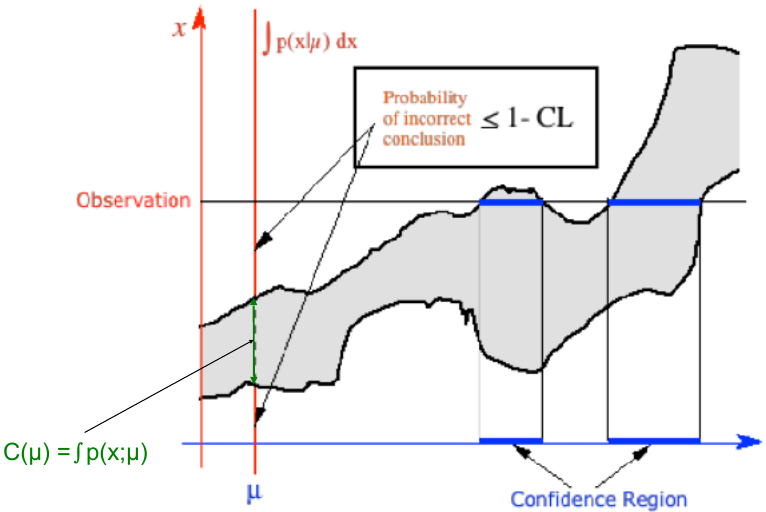
\includegraphics[width=0.9\textwidth,keepaspectratio]{clband}
    \label{fig:clband}
\end{figure}
\begin{figure}
    \centering
    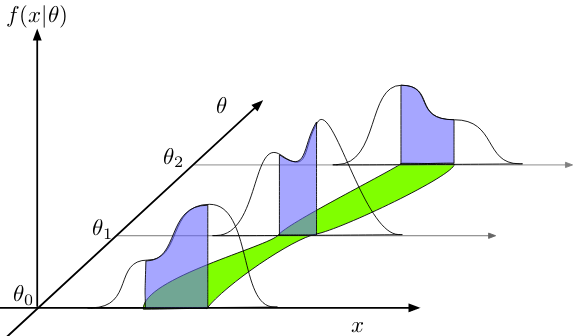
\includegraphics[width=0.9\textwidth,keepaspectratio]{neyman}
    \label{fig:neyman}
\end{figure}
\end{column}
\begin{column}{0.6\textwidth}
\begin{block}{Costruzione di Neyman}
Coverage: $\coverage{(\mu)}=\int_{x:\mu\in f(x)}\prob{(x:\mu)}\,dx$, $f(x)$ associa un intervallo nello spazio dei parametri a una misura; l'algoritmo ha livello di confidenza $\cl=\inf_{\mu\in A}C(\mu)$ cio\'e l'intervallo associato alla data misura ha probabilit\'a $\cl{}$ di contenere il parametro.
\end{block}
\begin{block}{Ordering}
''The way I integrate over the data''
\end{block}
\end{column}
\end{columns}
\end{frame}

\begin{frame}{Feldman-Cousins unified approach.}
\begin{columns}[T]
\begin{column}{0.5\textwidth}
insactisfaction with Neyman construction for upper limit in case of empty/unphysical interval (flip-flop problem depending on data)
\end{column}
\begin{column}{0.5\textwidth}
LR-ordering $R=\frac{\prob{(x;\mu)}}{\prob{(x;\mu_{best})}}$: values of x/n are added to acceptance region as decreasing function of R.
\end{column}
\end{columns}
\end{frame}

\subsection{Pivotal quantities}

\begin{frame}{Pivot}
Pivot: RV $U(T,\theta)$ funzione dib statistica sufficiente e parametro ma la distribuzione di U non dipende dal parametro $\forall \theta\in\Theta$ (asymptotic if true for $n\to\infty$).
\begin{align*}
&p(x;\mu)=\frac{1}{\sqrt{2\pi}\sigma}\exp{-\frac{(x-\mu)^2}{2\sigma^2}}\\
&(s=\frac{x-\mu}{\sigma}:\ p(s;\mu)=N(0,1)\\
&\int_{s>c}p(s)\,DS=\cl{}
\end{align*}
\mykeyword{Pivot. 2-sided CI for exponential}:
\begin{align*}
&f(x;\theta)=\invers{\theta}\exp{-\frac{x}{\theta}}I(x>0)\ \to\ g(u)=\exp{-u}I(u>0)\\
&\prob{(a<u<b)}=1-\alpha\Rightarrow\prob{(\theta\in(\invers{b}x,\invers{a}x))}=1-\alpha\ (\alpha\leftrightarrow1-\alpha)\\
&
\end{align*}
\end{frame}

\begin{frame}{Teorema di Wilks}
$p(x;\mu)$ due volte differenziabile con dominio indipendente da parametro $\Omega(x;\mu)=\Omega(x)$: \[\lambda(x;\mu)=2\log{[\frac{\sup_{\mu}{p(x;\mu)}}{p(x;\mu)}]}\] (log-likelihood ratio statistics) ha asintoticamente pdf universale e indipendente da $\mu$: distribuzione di $\chi^2$ con dof pari a dimensione di $\vec{\mu}$.
\begin{align*}
&\ln{L(\theta)}-\ln{L(\hat{\theta})}=-\frac{1}{2}\invers{F}_{\chi_n^2}(1-\alpha)
\end{align*}
\end{frame}

\begin{wordonframe}{Esempi intervalli di confidenza e credibilit\'a}
\begin{block}{Limite superiore Poisson con $k=0$}
$\prob{(k|\mu)}=\frac{\mu^k\exp{-\mu}}{k!}$: registro $k=0$ conteggi, ricavo limite superiore frequentista e bayesiano per $\mu$
\begin{columns}[T]
\begin{column}{0.5\textwidth}
\mykeyword{Ex: limite superiore bayesiano per Poisson} - La posterior $\prob{(\mu|0)}=\exp{-\mu}$ per $\cl{}=\alpha\%$ si ha $\int_0^{\mu_u}\exp{-\mu}\,d\mu=\alpha$, per $\cl{}=90\%$ si ha $\mu<2.3@90\%\cl{}$.
\end{column}
\begin{column}{0.5\textwidth}
\mykeyword{Ex: limite superiore bayesiano per Poisson} - 
\begin{picture}(100,130)
\put(20,20){
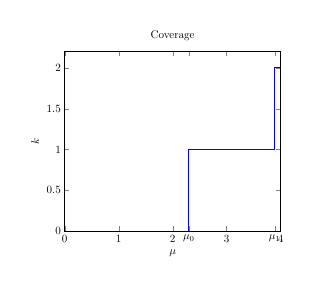
\begin{tikzpicture}[scale=0.4]
        \begin{axis}[title={Coverage},name=central,samples=50,ymin=0,xmin=0,xmax=4,xlabel={$\mu$},ylabel={$k$},extra x ticks={2.3,3.89,5.32},
    extra x tick labels={$\mu_0$, $\mu_1$, $\mu_2$}]
        \addplot+[const plot, no marks, thick] coordinates {(0,0) (2.3,1) (3.89,2) (5.32,3)};
        \end{axis}
    \end{tikzpicture}}
\end{picture}
\end{column}
\end{columns}
$\mu_0=\ln{10}$, $\mu_1: \prob{(0|\mu_1)}+\prob{(1|\mu_1)}=0.1$
\end{block}
\end{wordonframe}

\section{Test di ipotesi}
